\section{Results}\label{sec:results}

In this paper, we designed a new interpretability technique which can be used to extract knowledge graphs from state clouds of contextual embeddings. We have noticed that NSC is able to successfully recover commonsense relations of abstraction from raw text data (e.g. "apple" IS\_A "fruit", "orange juice" IS\_A "juice", see Fig. \ref{fig:nsc_output_graph}). Additionally, we have found that for a limited number of concepts to relate, the graph search is robust with respect to the starting state. Moreover, the legibility terms included in the linear combination which comprise the search objective (e.g. arc count) successfully nudge the search towards relatively sparse outputs. Finally, the graph search history profile exhibits proper foraging behavior, with fast increases in solution quality in the beginning, followed by a more conservative strategy which ends in marginal improvements towards the move to heavy exploitation (see Fig. \ref{fig:nsc_score_history}).

\begin{figure}[h]
    \centering
    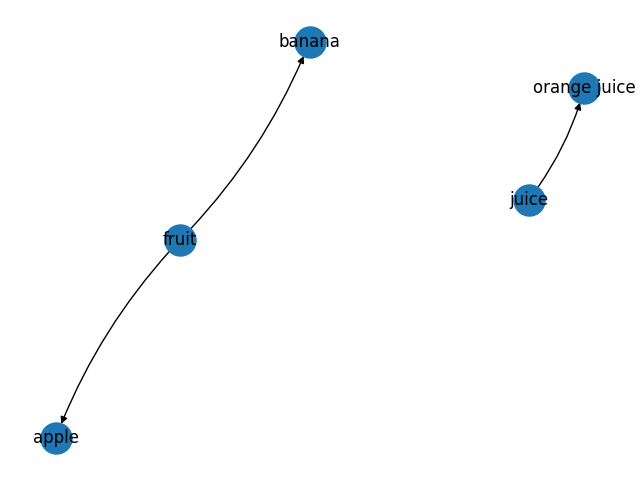
\includegraphics[width=0.45\textwidth]{img/distinct graphs.png}
    \caption{NSC output graph when applied to BERT using several symbols.}\label{fig:nsc_output_graph}
\end{figure}

\begin{figure}[h]
    \centering
    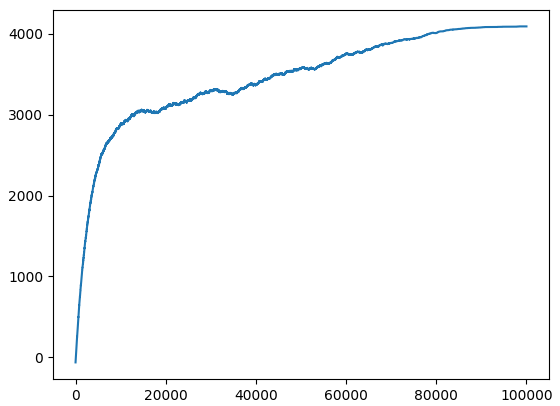
\includegraphics[width=0.45\textwidth]{img/score1.png}
    \caption{Candidate score by epoch during the local graph search.}\label{fig:nsc_score_history}
\end{figure}

\textbf{A graph optimization run with the same hyperparameter configuration and different targeted concepts resulted in a similar graph output (see Fig. \ref{fig:valuable}). Interestingly enough, while every single arc present in the output graph depicts a valid relation of abstraction (e.g. "food" $>$ "vegetable", "vegetable" $>$ "onion", etc.), the graph still has several shortcomings. The implicit structure of the concepts analysed would reflect the three vegetables mentioned (i.e. "carrot", "potato", and "onion") as children of the "vegetable" node. However, two of them (i.e. "carrot" and "potato") have been linked directly to the more abstract "food".}

\textbf{This likely reflects a limitation of the objective function we employed. Namely, the four terms of the linear combination (i.e. expressed abstraction, arc density, children error, and parent error) have collectively proven insufficient for capturing and incentivizing this implicit structure. It appears more valuable for the graph optimization algorithm in terms of the objective function to populate the graph with arcs which denote particularly \textit{abrupt} relations of abstraction. In this last graph output (see Fig. \ref{fig:valuable}), this is reflected in the favoring of the ("food", "potato") arc over the $\{("food", "vegetable"), ("vegetable", "potato")\}$ pair of arcs. Alternatively, arc density could be penalized less in order to render this arc pair more appealing in contrast to the single more abrupt arc.}

\begin{figure}[h]
    \centering
    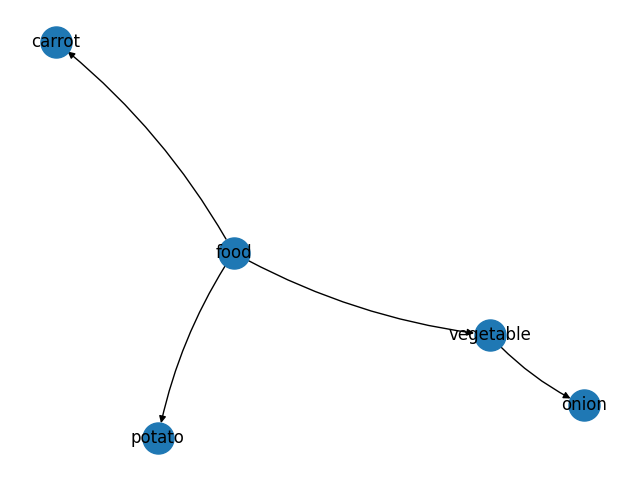
\includegraphics[width=0.45\textwidth]{img/valuable contrasts.png}
    \caption{NSC output graph when applied to BERT using several symbols.}\label{fig:valuable}
\end{figure}


- eigenvalue spectrum

\begin{figure}[h]
    \centering
    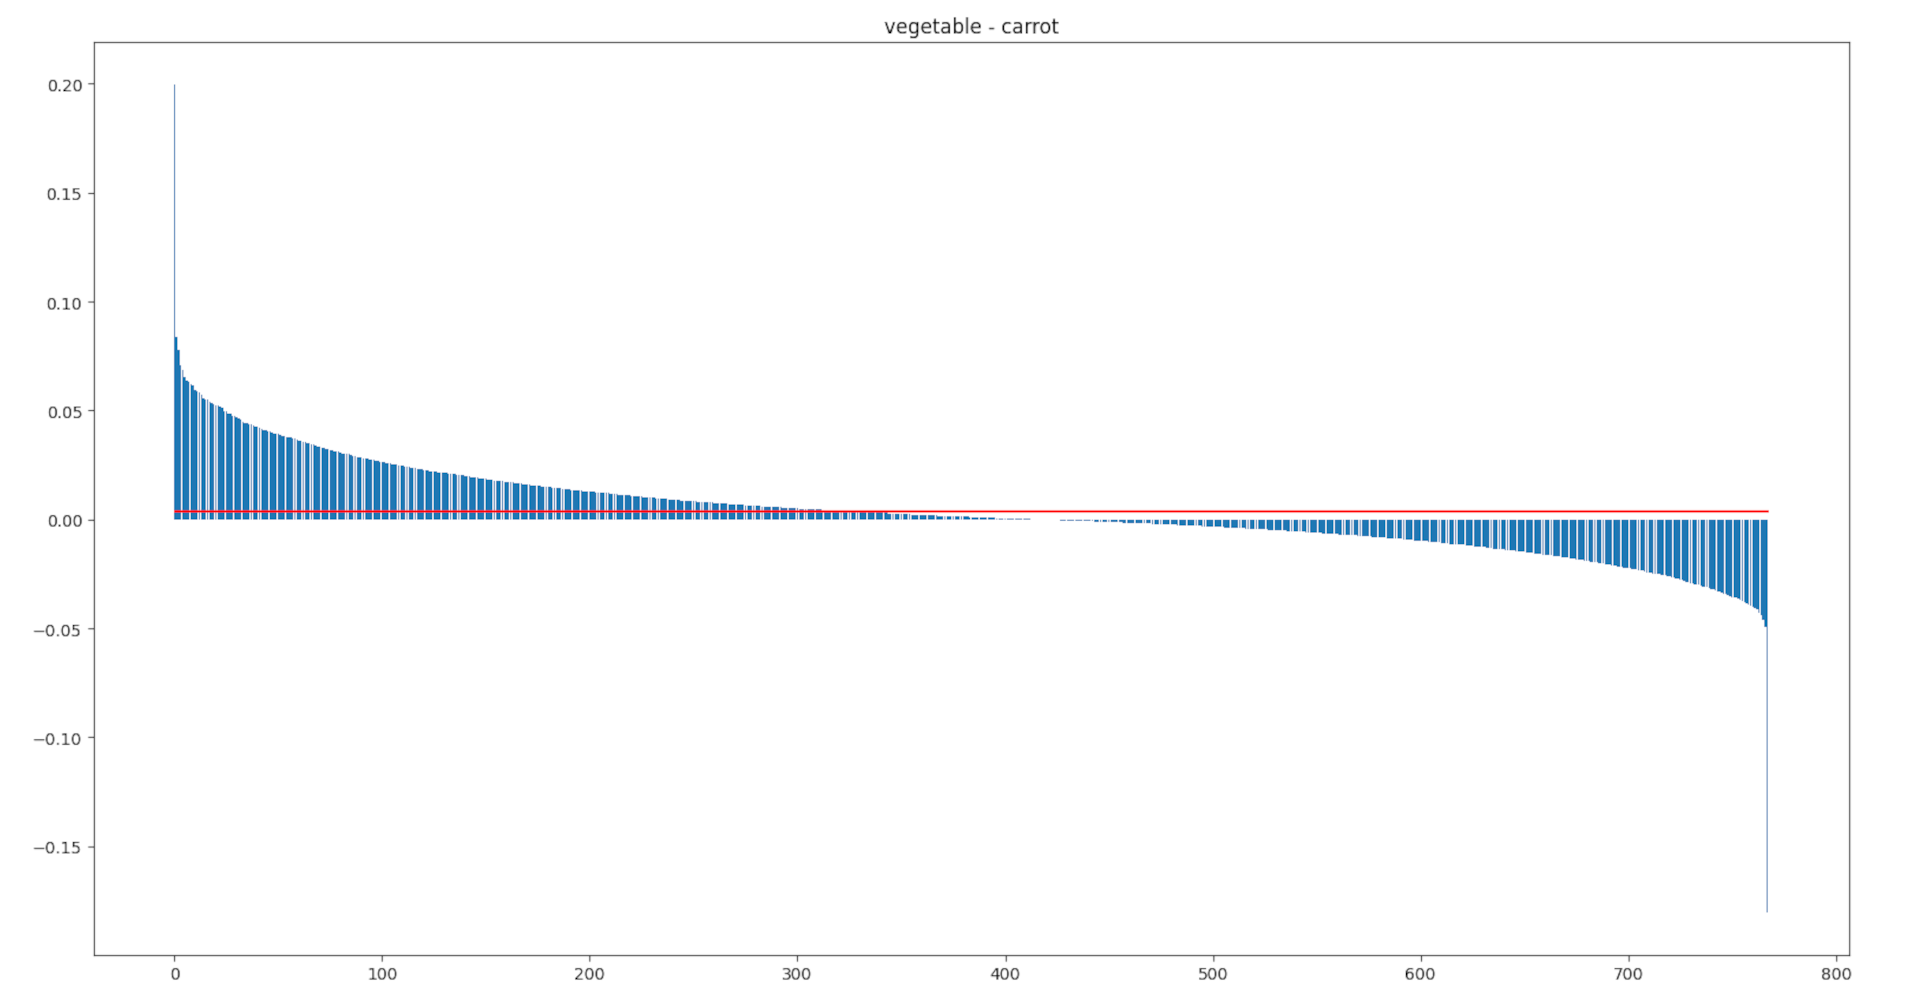
\includegraphics[width=0.45\textwidth]{img/spectrum.png}
    \caption{NSC output graph when applied to BERT using several symbols.}\label{fig:spectrum}
\end{figure}